\documentclass[12pt]{article}


\usepackage[english,italian]{babel} %lingue utilizzabili

%grafica
\usepackage{graphicx}
\usepackage{fancyhdr} %font
\usepackage{subfig}
\usepackage{float}

\usepackage[utf8]{inputenc} %codifica e input

\usepackage{hyperref} %indice linkato ai paragrafi di riferimento
\hypersetup{
  colorlinks,
  citecolor=gray,
  filecolor=brown,
  linkcolor=black,
  urlcolor=cyan
}

\usepackage{lastpage} %per sapere il numero di pagine totali

\usepackage{parcolumns} %testo affiancato in colonna

\usepackage{listings} %Per inserire codice
\usepackage[usenames]{color} %Per permettere la colorazione dei caratteri 

\usepackage[a4paper,top=3cm,bottom=2cm,left=2cm,right=2cm] {geometry} %imposta pagina formato A4 e setta margini a piacimento
\usepackage[pdftex]{lscape} %per settare pagine in landscape

\renewcommand{\familydefault}{\sfdefault}   %mette tutto il carattere con uno stile ''grazioso'' <-----------------------------------molto bello

\definecolor{editorGray}{rgb}{0.95, 0.95, 0.95}
\definecolor{editorOrange}{rgb}{1, 0.5, 0} % #FF7F00 -> rgb(239, 169, 0)
\definecolor{editorGreen}{rgb}{0, 0.6, 0} % #007C00 -> rgb(0, 124, 0)




%personalizzazione classe per il codice SQL
\lstnewenvironment{sql}[1][] 
{\lstset{basicstyle=\scriptstyle \ttfamily, columns=fullflexible, keywordstyle=\color{blue}\bfseries, ndkeywordstyle=\color{blue}\bfseries , ndkeywords={references}, numberstyle=\color{red}, commentstyle=\color{editorGreen}, showstringspaces=false, stringstyle=\color{editorOrange},
language=SQL, basicstyle=\small,
numbers=left, numberstyle=\tiny,
tabsize=2, stepnumber=10, numbersep=5pt, breaklines=true, frame=single, rulecolor=\color{black}, #1}}
{\lstset {language=SQL,morekeywords={INT,CHAR,varchar,smallint,numeric}}}{}


%personalizzazione classe per il codice HTML
\lstnewenvironment{html}[1][] 
{\lstset{basicstyle=\scriptstyle \ttfamily, columns=fullflexible,
keywordstyle=\color{blue}\bfseries, ndkeywords={content,=,charset=, id=, width=, height=},	 ndkeywordstyle=\color{editorGreen}\bfseries , numberstyle=\color{red} commentstyle=\color{red}, showstringspaces=false, stringstyle=\color{editorOrange},
language=HTML, basicstyle=\small,
numbers=left, numberstyle=\tiny,
tabsize=2, stepnumber=10, numbersep=5pt, breaklines=true, frame=single, rulecolor=\color{black}, #1}}{}

%personalizzazione classe per il codice PERL
\lstnewenvironment{perl}[1][] 
{\lstset{basicstyle=\scriptstyle \ttfamily, columns=fullflexible,
keywordstyle=\color{blue}\bfseries, ndkeywords={content,=,charset=, id=, width=, height=},	 ndkeywordstyle=\color{editorGreen}\bfseries , numberstyle=\color{red} commentstyle=\color{red}, showstringspaces=false, stringstyle=\color{editorGreen},
language=PHP, basicstyle=\small,
numbers=left, numberstyle=\tiny,
tabsize=2, stepnumber=10, numbersep=5pt, breaklines=true, frame=single, rulecolor=\color{black}, #1}}{}





\begin{document}

\begin{figure}
\centering

\includegraphics[angle=0]{img/logo.png}
\end{figure} 

\title{ \textbf{{\Huge SitesBoard}}\vspace{2cm} \\ {\Huge Tecnologie Web \\ Relazione del progetto} \\ {\Large Anno accademico 2015/2016} }
%\date{}
 
\author{
\begin{tabular}{r|l}
\textbf{Componenti} & Fasolato Francesco\\
&Macrì Antonino\\
&Rigoni Davide\\
&Zecchin Giacomo
\end{tabular}\vspace{0.5cm} \\
	Indirizzo Web: \\ \\ \url{http://tecnologie-web.studenti.math.unipd.it/tecweb/~drigoni}\vspace{0.3cm} \\
	Email responsabile: \href{mailto:davide.rigoni.2@studenti.unipd.it}{davide.rigoni.2@studenti.unipd.it} 
}

\maketitle
\thispagestyle{empty}


\newpage


%da qui stile intestazione e piè di pagina cosi definiti
\pagestyle{fancy}
\lhead{}
\lfoot{\emph{\large SitesBoard}} 
\cfoot{}
\rfoot{Pagina: \thepage\ di \pageref{LastPage}}
\renewcommand{\footrulewidth}{0.5pt}
%%%%%%%%%%%%%%%%%%%%%%%%%

\tableofcontents %CREA INDICE



\newpage

\section{Abstract}
Come suggerisce il nome, SitesBoard è una bacheca digitale contenente inserzioni che offrono opportunità lavorative concernenti la realizzazione di siti web.

SitesBoard permette agli utenti registrati al suo interno di inserire nuovi annunci oppure accettare quelli proposti da altri utenti.
Ogni utente ha un’area personale, nella quale sono presenti i propri dati profilo e da quest’area può accedere alla pagina degli annunci che ha inserito o a quella degli annunci che ha accettato.
Per ogni annuncio proposto, è visibile la lista degli utenti che hanno dato la loro disponibilità. 

Spetta a chi l’ha pubblicato cancellare l'inserzione quando lo desidera e contattare il candidato che ritiene essere più adatto per il lavoro.
Gli annunci sono divisi in categorie per aiutare gli sviluppatori a trovare quelli più adatti alle loro abilità. 

Le categorie sono: E-commerce, Forum, Social, Personali, Aziendali e Blog.
In ogni categoria gli annunci appaiono all’utente ordinati secondo la data di inserimento.

%\selectlanguage{italian}	%%%%inserirlo causerebbe errore in compilazione per lettere accentate-->non risolto


\section{Utenti destinatari}
Il nostro sito si rivolge ad un’utenza formata sia da utenti abbastanza abili nell’uso di linguaggi di programmazione, sia da utenti che non hanno molte conoscenze informatiche e che, proprio per questo, usufruiranno del nostro servizio digitale per contattare qualcuno in grado di realizzare un sito web.
\newpage

\section{Progettazione}
	\subsection{Struttura}
		\subsubsection{Organizzazione cartelle}
		
		I file che compongono il sito sono organizzati su 3 cartelle:

		\begin{itemize}

			\item \textbf{public\textunderscore html}: contiene le pagine statiche, gli stili, il codice javaScript e le immagini contenute nel sito;
			\item \textbf{data}: contiene i files accessibili solo internamente al server, quindi i file xml, i fogli di trasformazione e la definizione dello schema;
			\item \textbf{cgi-bin}: contiene gli script cgi o più precisamente perl che generano dinamicamente le pagine del sito.

		\end{itemize}


		\subsubsection{Definizione}
	
		Il sito visualizzabile da un utente comune non registrato/loggato si compone principalmente di 11 pagine:
		
		\begin{itemize}
			\item \textbf{home.cgi}: È la homepage del sito; mostra gli annunci di tutti gli utenti in ordine di data.
			\item \textbf{pagine suddivise per le diverse categorie di annunci}: Le pagine eCommerce.cgi, forum.cgi, social.cgi, personali.cgi, aziendali.cgi e blog.cgi mostrano gli annunci della loro tipologia.
			\item \textbf{registration.cgi}: È la pagina che contiene la form per la registrazione al sito di SitesBoard.
			\item \textbf{login.cgi}: È la pagina che contiene la form per eseguire la login al sito.
			\item \textbf{pass\textunderscore recovery.html}: È la pagina che contiene la form per il recupero della password utente eventualmente dimenticata.\\
			\item \textbf{insertion.cgi}: È la pagina che permette di visualizzare i dati delle inserzioni.
		\end{itemize}
		Le pagine aggiuntive alle quali hanno accesso solamente gli utenti che hanno effettuato il login sono 6:
		
		\begin{itemize}
			\item \textbf{profile.cgi}: È la pagina che mostra i dati personali dell'utente che ha effettuato il login.
			\item \textbf{profileChange.cgi}: È la pagina che contiene la form per la modifica dei dati personali dell'utente.
			\item \textbf{addInsertions.cgi}: È la pagina che contiene la form per l'inserimento di un nuovo annuncio.
			\item \textbf{showInsertions.cgi}: È la pagina che mostra gli annunci che ha inserito l'utente.
			\item \textbf{acceptedInsertions.cgi}: È la pagina che mostra gli annunci accettati dall'utente.
			\item \textbf{userProfile.cgi}: È la pagina che mostra i dati di un altro utente registrato al sito.
		\end{itemize}
		
	
		\subsubsection{Database}
		Il database è stato realizzato utilizzando un unico file chiamato “database.xml”.
		Avremmo potuto infatti dividere il nostro database in 2 file distinti, ad esempio “utenti.xml” e “annunci.xml”.
		La nostra scelta è stata dovuta alla maggiore praticità nel gestire un singolo file e al fatto che interrogare più database in quasi tutte le query sarebbe stato troppo dispendioso.\\
		Il file è stato strutturato seguendo il modello a bambole russe e motivazioni che hanno portato a questa scelta sono dovute alle caratteristiche di questo modello:
		
		\begin{itemize}
			\item Semplifica la leggibilità della struttura poiché rispecchia la struttura del documento XML.
			\item Ogni tipo complesso ha una struttura diversa dagli altri tipi complessi perciò ogni elemento è definito localmente.
		\end{itemize}
		
		La struttura del documento XML è stata definita con XML Schema poiché esso fornisce una descrizione più dettagliata di quella che avrebbe potuto definire un file DTD.

	\subsection{Presentazione}
	
	Il sito è impostato secondo un layout ibrido a 3 pannelli in cui le dimensioni del testo e delle altezze dei blocchi sono date in ems, mentre la larghezza è data in \% secondo la dimensione della pagina.
	
	Per una maggiore usabilità sono presenti due differenti visualizzazioni del sito, a seconda del dispositivo utilizzato per la navigazione.
	È stato impostato un punto di rottura a 800px di larghezza al di sotto del quale si passa da una visualizzazione desktop ad una adatta per dispositivi mobile o tablet con piccoli schermi.
	
	A sinistra c'è il menù di navigazione che permette all’utente di raggiungere varie sezioni del sito in base al suo interesse, in alto l'header e la breadcrumb, nella zona centrale il corpo del contenuto ed infine in basso il footer.
	Per quanto riguarda il layout ridotto, esso si sviluppa in verticale. Dall’alto verso il basso si trovano in ordine header, breadcrumb, il menù di navigazione, il corpo e il footer.
		
	E\' stato scelto di usare gli ems in modo da permettere che il testo si adatti alle dimensioni decise dall'utente.
	Dobbiamo anche considerare la non scalabilità dei pixel in IE nei browser più vecchi. Se un un utente ha bisogno di ingrandire le dimensioni di tutto il sito il font settato in pixel rimane della stessa dimensione creando gravi problemi di accessibilità poiché molti utenti con problemi alla vista non riuscirebbero ad accedere ai contenuti.
	Anche gli ems però presentano un piccolo svantaggio che è quello di dover considerare il contesto in cui si trovano se vogliamo mantenere un testo reattivo.\\ Visto che il contenuto di SitesBoard è rappresentato quasi unicamente da testo (sono presenti solo 3 loghi nell'header) il problema di gestire le immagini durante il ridimensionamento di quest'ultimo diventa irrilevante.
	
	Il layout così impostato diventa molto fluido, accessibile ed adattabile ad ogni dispositivo di navigazione e ciò sta alla base di un responsive layout.
	
	\newpage
	
	
	\begin{figure}
 		\begin{minipage}[b]{8.5cm}
  		 \centering
   		
\includegraphics[angle=0,scale=.7]{img/layout1.png}
   		\caption{Visualizzazione Desktop}
 		\end{minipage}
 	\ \hspace{2mm} \hspace{3mm} \
		 \begin{minipage}[b]{8.5cm}
  		\centering
   		
\includegraphics[angle=0,scale=.7]{img/layout2.png}
   		\caption{Visualizzazione Mobile}
 		\end{minipage}
	\end{figure}
	
	\subsection{CSS}
	
	Il footer è fissato sempre in fondo alla pagina tramite una tecnica che sfrutta solo CSS, in quanto imposta ai blocchi solamente le proprietà "margin" e "height". \\
	Tende ad essere retrocompatibile e funziona anche su Internet Explorer 6.\\

	
	\subsection{Javascript}
	
	Il linguaggio javascript è stato utilizzato per i controlli degli input delle form in locale.
	I controlli fatti sono di due tipi: 
	Javascript è stato usato anche per rendere migliore l'esperienza del sito con il conta caratteri, la funzione di svuotamento di un campo input di changeProfile.cgi che viene in automatico precompilato con valori di default presi da quelli precedentemente inseriti e una funzione di richiamo di un alert di avvertimento in caso di click alla form di elimina del proprio profilo.
	
	\subsection{Perl}
	
	Gran parte delle pagine del nostro sito sono state realizzate con PERL per sfruttare la possibilità di effettuare sempre i controlli sull’identità dell’utente.
	
	Il tempo di permanenza di un utente su una singola pagina è limitato a 60 minuti. Se l’utente non cambia pagina entro quel limite di tempo, la sessione scade e gli viene chiesto di nuovo di effettuare il log-in. \\	
	Le pagine PERL che vengono utilizzate solo come pagine di transizione per effettuare controlli o dialogare col database sono le seguenti:	
	"addAcception.cgi", "addUser.cgi", "changeUserData.cgi", "checkLogin.cgi", "insertInsertions.cgi", "logout.cgi", "recoveryUser.cgi", "removeAcception.cgi", "removeInsertion.cgi", "removeProfile.cgi".
	
Le pagine di scrittura dati nel database, “addAcception.cgi” e “addUser.cgi”, “changeUserData.cgi" e “insertInsertion.cgi", prima di tutto effettuano i controlli di routine per verificare se l’utente che effettua l’operazione è presente nel database. Una volta superati i controlli si verifica se anche l’annuncio sul quale si vuole operare sia disponibile e poi, sempre grazie ai percorsi xPath e a funzioni apposite (come “findnodes( )” e “appendChild( )" ), si va ad effettuare la modifica del file “database.xml”.

Per garantire la solidità del database, nel file “addUser.cgi” si va anche ad effettuare una ricerca dell'attributo “persona/id” di tutti gli utenti già presenti nel database. Una volta trovati tutti si ricerca quello con valore più alto e si garantisce che il nuovo utente abbia il più piccolo valore intero che supera il valore appena trovato.

Le pagine di rimozione dati nel database, “removeAcception.cgi”, “removeInsertion.cgi” e “removeProfile.cgi”, sono duali a quelle di inserimento dati, tranne per il fatto che sfruttano la funzione removeChild( ).

La pagina “recoveryUser.cgi”, usata per recuperare la password dell’utente, effettua dei controlli sul database di:
Nome, Cognome, Data di Nascita, Username, E-mail.\\
Se l’utente inserisce correttamente tutti i dati ed inserisce una nuova password, questa viene sovrascritta alla precedente nel database. La modalità di recupero password così implementata impedisce ogni tentativo di impossessarsi di un account altrui, poiché i dati di ogni utente visibili da tutti gli altri all’interno del sito sono solo: Username e E-mail ( è disponibile anche il campo Biografia, che non viene richiesto nella procedura del recupero password per ovvi motivi).

La pagina “checkLogin.cgi” effettua i controlli sui parametri passati, ovvero verifica se Username e Password sono corretti, nel caso in cui non lo siano, l’utente viene reindirizzato alla pagina “Login.cgi”, mentre se sono corretti, è possibile accedere alla pagina del proprio profilo personale “profile.cgi”. Se un utente vuole tentare di bypassare la procedura di log-in accedendo ad una pagina tramite url, la pagina “checkLogin.cgi” lo reindirizza alla home del sito.

La pagina “logout.cgi” si occupa di chiudere l’eventuale sessione tramite il metodo “destroySession( )” e reindirizza alla home.
	
	\subsection{XSLT}
	
	Abbiamo realizzato una versione più “semplice” della home del nostro sito usando XSLT. Questa pagina è stata pensata per essere utilizzata da utenti che non hanno effettuato il login. Infatti vengono visualizzati solo gli annunci presenti nel nostro database, come nel file “home.cgi", ma con alcune differenze.

Per quanto riguarda gli annunci stessi vengono visualizzati: Titolo, Oggetto, Tipologia di Annuncio, la data in cui sono stati inseriti e la descrizione. Tutti i campi sono ordinati per data descrescente. Abbiamo evitato volontariamente di fornire all’utente non registrato (o che non ha ancora effettuato il log-in) le informazioni che riguardano l’utente che ha inserito l’annuncio, per evitare che possa usufruire delle funzionalità del nostro sito, mettendosi in contatto con lui.

E’ stato realizzato il foglio di stile "screen\textunderscore xsl.css” apposito per "home.xsl", per rendere più gradevole l’aspetto della pagina. E’ stata realizzata solo la visualizzazione screen come esempio. 
Purtroppo per ragioni logistiche di organizzazione delle cartelle e dei file, non abbiamo potuto aprire questo file dal server e così abbiamo deciso di tenerlo solo come esempio, per essere visualizzato in locale.


\section{Accessibilità}
Il sito è stato pensato per essere facilmente consultabile dalla maggior utenza possibile, anche se è rivolto ad un pubblico con una esperienza medio-alta nell’uso di internet.

Per chi dovesse aver disabilitato, volontariamente o meno, JavaScript, sono state scritte le funzioni principali che controllano l’input dalle form con il linguaggio PERL. Le scelte effettuate per adempiere a tali propositi sono spiegate a seguire.

	\subsection{Struttura}
	
\begin{itemize}
	\item Uso di attributo “alt” per ogni immagine presente in modo da fornire un’alternativa testuale per contenuti non testuali.
	\item Si cerca di mantenere la stessa struttura in tutte le pagine ( fatta eccezione per “home.xsl” che è stata realizzata solo per esempio e per essere vista in locale ) per evitare di disorientare l’utente. 
	\item Uso dell'attributo “xml:lang” e “lang” per identificare le parole in lingua straniera, in modo che uno screen reader possa leggerle correttamente, come specificato nel documento (\url{https://www.w3.org/TR/REC-xml/}). L’attributo non è presente solamente all’interno dei tag “title”, poiché, come da specifiche W3C, non è possibile inserire un tag “span” all’interno di un “title”.
	\item Le pagine Web hanno titoli che ne descrivono l’argomento o la finalità.
	\item Tutti i contenuti più importanti sono identificati dall’attributo “title” che ne specifica l'argomento.
	\item Sono stati utilizzati tutti colori “web safe”, ovvero colori compatibili con tutti i browser, recenti o meno.
	\item Uso di tabindex nelle form per permettere una navigazione facilitata attraverso l’uso della sola tastiera. Sono stati realizzati associando al primo field della form l’indice “1” in modo da dare priorità al contenuto della pagina, rispetto al menù laterale.
	\item All’inizio di ogni pagina è stato dato fornito un link, permettendo così agli utenti che fanno uso di uno screen reader di saltare direttamente al contenuto della pagina, senza perdita di tempo.
	\item Ogni form è caratterizzata da un titolo. Tutti i field delle form sono stati dotati di una label e le voci sono state raggruppate tramite fieldset.
	\item Non sono state usate tabelle, tutte le strutture sono state realizzate tramite div e liste.
	\item Il pulsante di elimina profilo presente nella pagina “profile.cgi" rimanda alla pagina “confirmRemoveProfile.cgi" che funziona anche senza JavaScript e richiede la conferma dell’eliminazione del profilo.
	\item L'intero sito è stato strutturato per essere completamente utilizzabile anche con JavaScript disabilitato.
	\item Le piccole icone in altro a destra associate al profilo, alla modifica profilo e al logout sono caricate tramite CSS e non dall'html poiché non sono informazioni aggiuntive al contenuto; inoltre velocizzano il caricamento del sito.
	\item Le immagini presenti nel nostro sito sono state riadattate alla dimensione nella quale vengono visualizzate, per velocizzare il download delle componenti del sito.
\end{itemize}
	
	\subsection{Visualizzazione}
	Di seguito è riportata l'anteprima standard della pagina ''profile.cgi'':
	
	\begin{figure}[H]
	\centering
     		 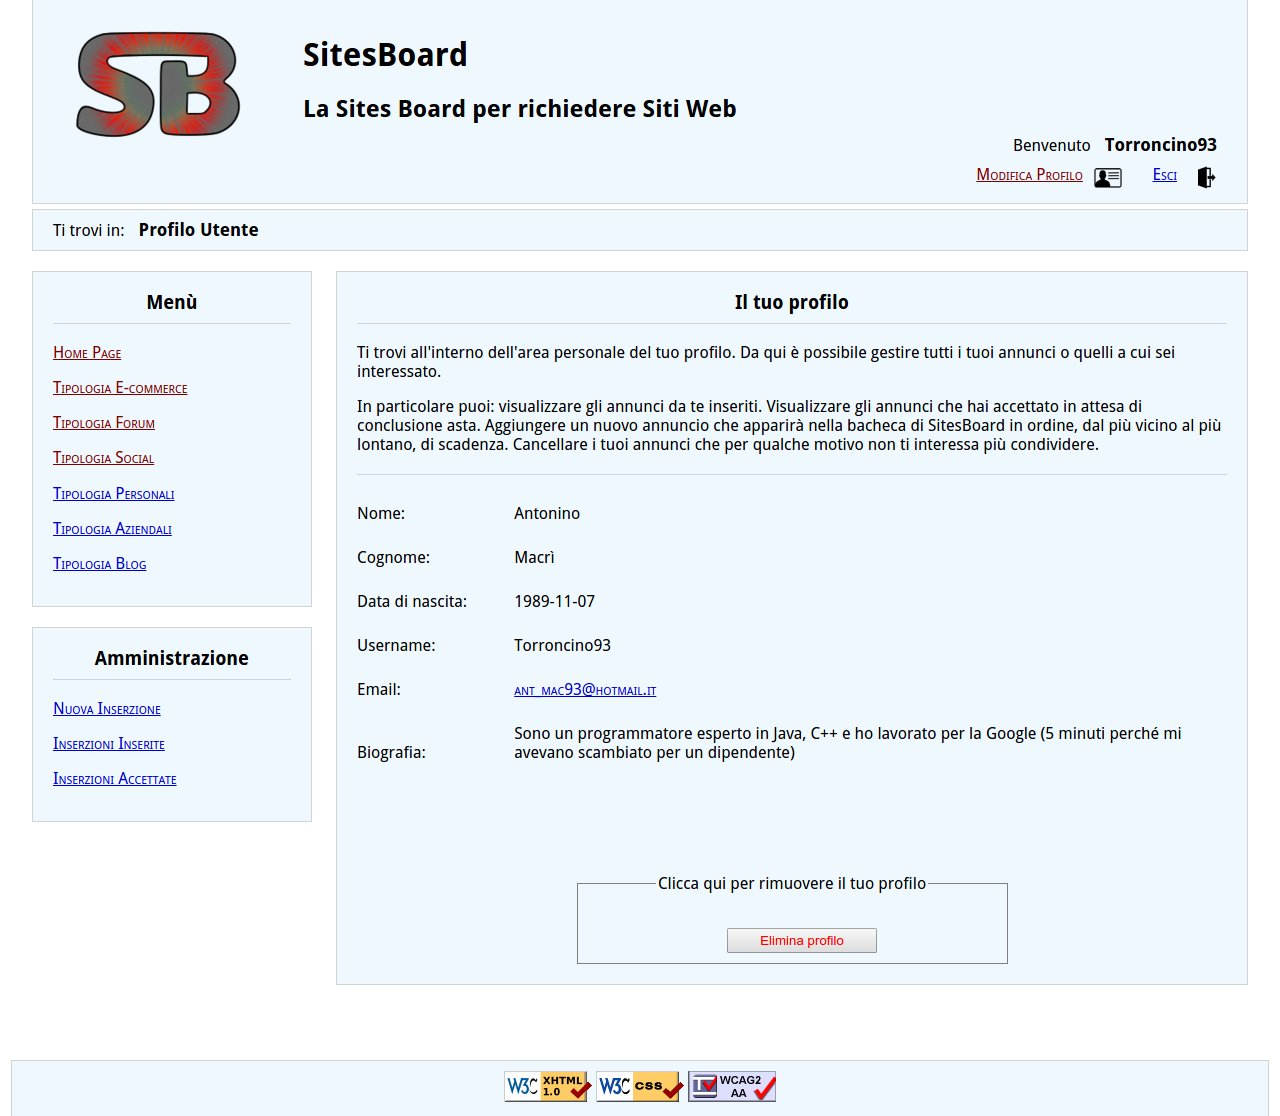
\includegraphics[scale=0.3]{img/userProfile_SitesBoard.jpg}
		 \caption{Anteprima standard ''Profile.cgi''}
	\end{figure}
	
	Evidenziamo alcune caratteristiche visive che aumentano l'accessibilità del sito:
	
\begin{itemize}
	\item I paragrafi di testo soddisfano i seguenti requisiti:
		\begin{itemize}
		\item Lo spazio tra i paragrafi è almeno una volta e mezzo più grande rispetto all’interlinea. (w3c AAA)
		\item Il testo su tutti i contenuti non è giustificato per renderlo più leggibile. (w3c AAA)
		\item Il testo può essere ridimensionato fino al 200\% in modo che non venga richiesto all'utente lo scroll orizzontale per leggere quella che sarebbe stata un'unica riga di testo nella visualizzazione full-screen. (w3c AAA)
		\end{itemize}
	\item  I componenti che hanno la stessa funzionalità all’interno di un insieme di pagine web sono identificati in modo univoco. (ad esempio nav\textunderscore menu, nav\textunderscore login ecc.)
	\item I componenti di ogni pagina del sito sono accessibili anche solo tramite l'input da tastiera.
	\item Non sono presenti lampeggi del monitor dovuti ad immagini o testi animati che potrebbero essere pericolosi per le persone affette da epilessia fotosensibile.
\end{itemize}
	
	

	\subsection{Comportamento}
	Riportiamo gli aspetti tecnici più rilevanti del nostro sito:
	
	\begin{itemize}
	\item Controlli lato server realizzati con PERL per sopperire alla mancanza di Javascript qualora un utente l'avesse disabilitato.
	\item Degradazione elegante con JavaScript assente o disabilitato.
	\end{itemize}

	\newpage
	
	\subsection{Test effettuati}
		\subsubsection{Conformità standard WCAG}
		
		Tutte le pagine HTML generate dalle nostre pagine .cgi sono state testate all'indirizzo \url{url} [......]
		\subsubsection{Contrato testo e sfondo}
		
		I test sono stati effettuati con Colour Contrast Analyser, reperibile a questo indirizzo: \url{http://www.paciellogroup.com/resources/contrastanalyser/}.\medskip
		
Affinché il contrasto possa ottenere una valutazione di tripla A secondo le norme del W3C, devo avere una soglia minima garantita di: differenza di colore:500 / differenza di luminosità:125.\\
Le combinazioni di testo e sfondo possibili sono le seguenti:

\begin{itemize}
\item Sfondo bianco (\#FFFFFF), Testo nero (\#000000) per alcuni pulsanti: ottiene un punteggio di tripla A per quanto riguarda il testo  piccolo, che è quello che viene utilizzato sul sito. differenza di colore:765 / differenza di luminosità:255.
\item Sfondo azzurro chiaro (\#ECF6FE), Testo nero (\#000000) utilizzato per la maggior parte del testo presente nel nostro sito: ottiene un punteggio di tripla A sia per quanto riguarda il testo grande, che quello piccolo. differenza di colore:736 / differenza di luminosità:243.
\item Sfondo azzurro chiaro (\#ECF6FE), Testo blu (\#0000CD) utilizzato per i link a pagine non ancora visitate del nostro sito: ottiene un punteggio di tripla A per quanto riguarda il testo piccolo, che è quello che viene utilizzato sul sito. differenza di colore:531/ differenza di luminosità:220.
\item Sfondo azzurro chiaro (\#ECF6FE), Testo viola (\#800000) utilizzato per i link a pagine già visitate del nostro sito: ottiene un punteggio di tripla A sia per quanto riguarda il testo grande, che quello piccolo. differenza di colore:608/ differenza di luminosità:205.
\item Sfondo azzurro chiaro (\#ECF6FE), Testo rosso (\#FF0000) utilizzato per visualizzare i messaggi d'errore del nostro sito: ottiene un punteggio di tripla A per quanto riguarda il testo piccolo, che è quello che viene utilizzato sul sito. differenza di colore:519/ differenza di luminosità:167.
\item Sfondo azzurro chiaro (\#ECF6FE), Testo verde (\#228B22) utilizzato per visualizzare i messaggi di successo del nostro sito: ottiene un punteggio di tripla A per quanto riguarda il testo piccolo, che è quello che viene utilizzato sul sito. differenza di colore:529/ differenza di luminosità:148.
\end{itemize}
		
		\subsubsection{Screen reader}
		
		Sono stati effettuati dei test con lo screen-reader “NVDA” su sistema operativo Windows 7 per verificare che SitesBoard fosse accessibile anche all’utenza con disabilità visiva. 
		
		\subsubsection{Disturbi visivi}
		
		Sono state effettuate simulazioni per quanto riguarda la visione del sito da parte di persone affette da disturbi visivi quali Protanopia, Deuteranopia, Tritanopia. Si allegano le immagini che dimostrano come il sito sia accessibile anche per queste categorie di persone.
	\vspace{2cm}
	
	\begin{figure}[H]
	\centering
    		\subfloat[Protanopia\label{Protanopia}]{%
     		 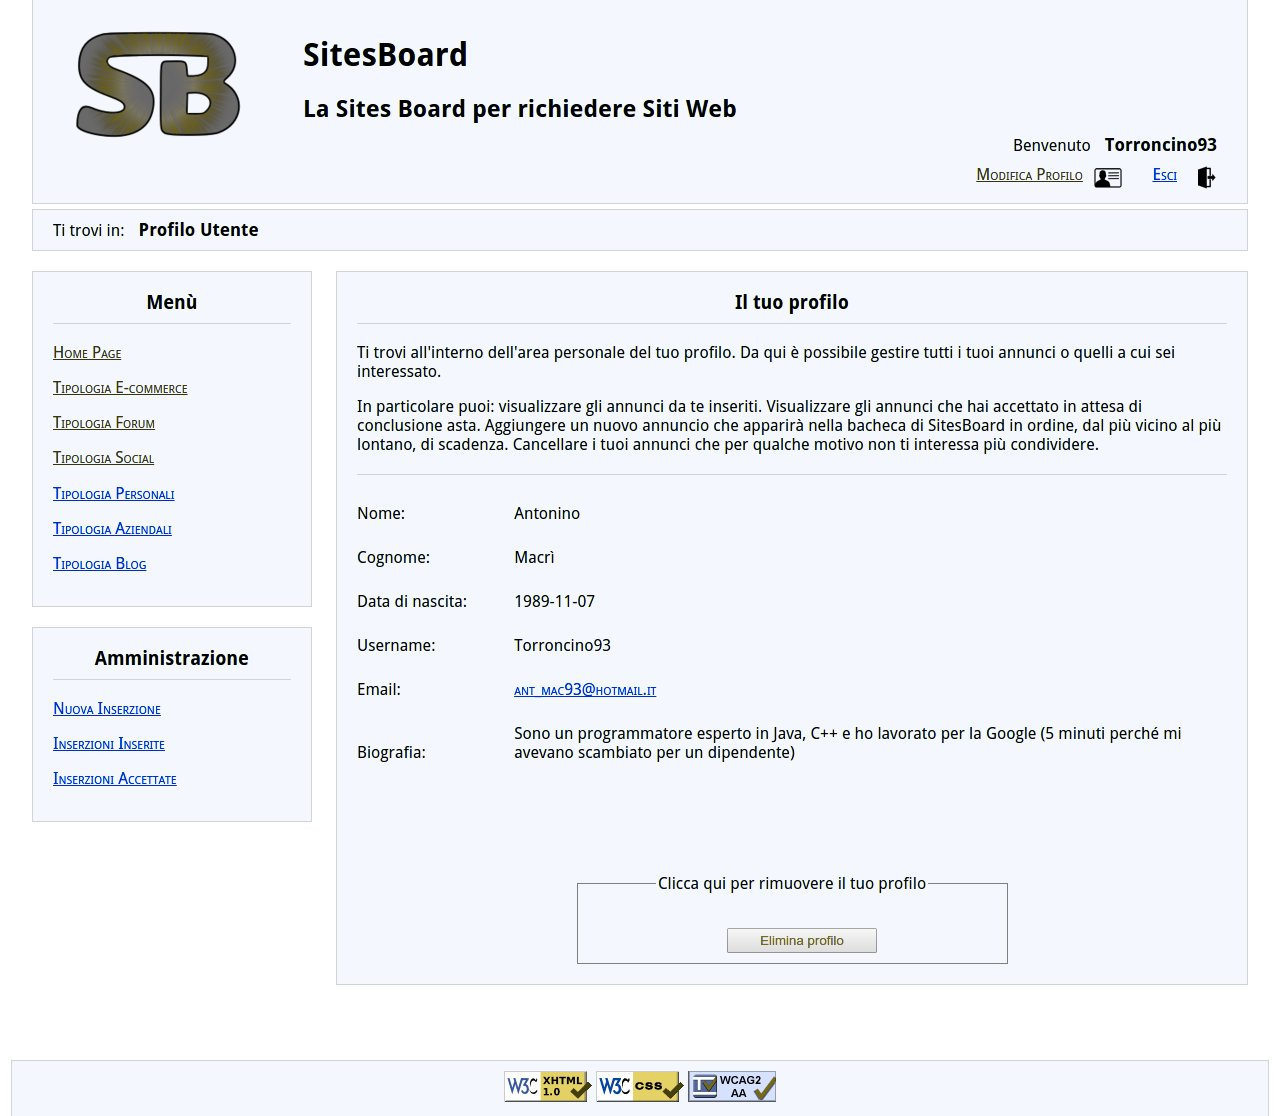
\includegraphics[scale=0.3]{img/userProfileProtanope_SitesBoard.jpg}
   		 }
	\end{figure}
   	
	\newpage
	
	\begin{figure}[H]
	\centering
    		\subfloat[Deuteranopia\label{Deuteranopia}]{%
     		 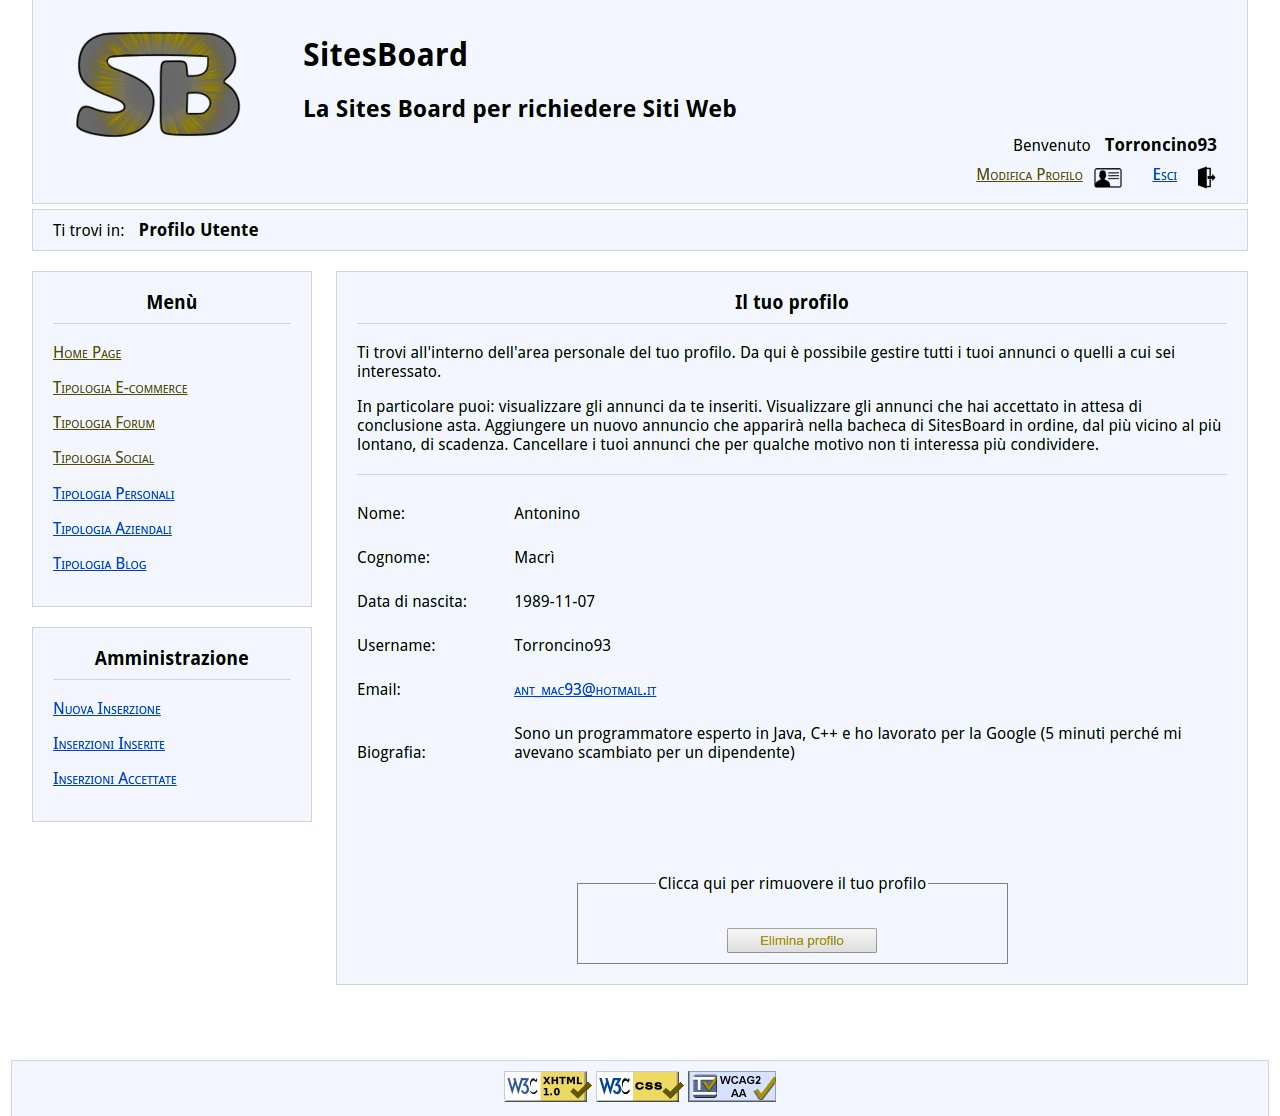
\includegraphics[scale=0.3]{img/userProfileDeuteranope_SitesBoard.jpg}
   		 }
   		 \vfill
    		\subfloat[Tritanopia\label{Tritanopia}]{%
      		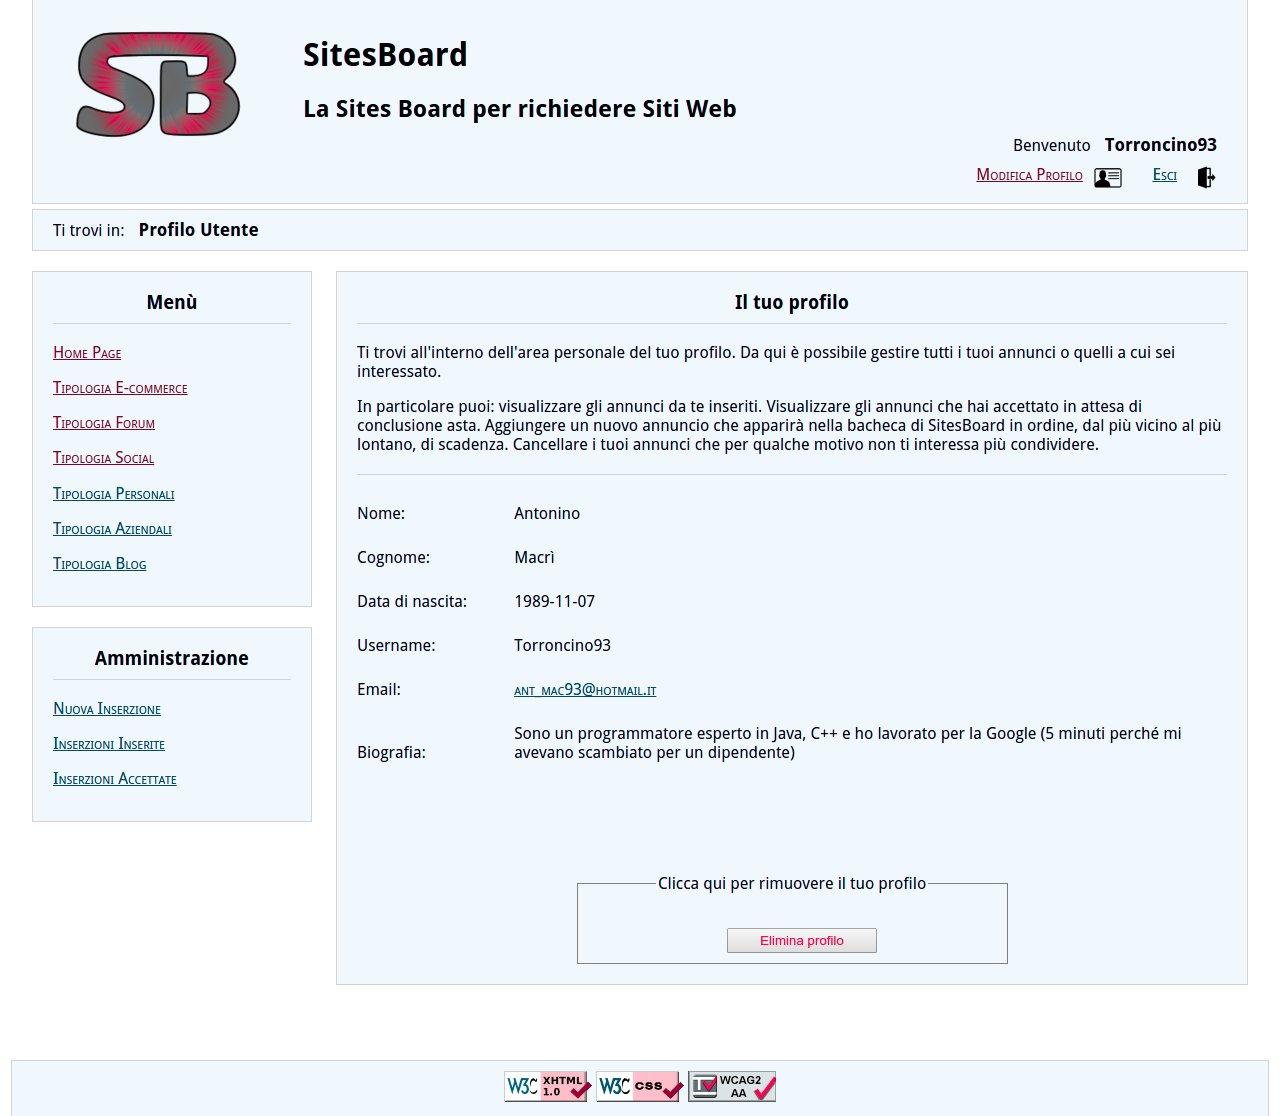
\includegraphics[scale=0.3]{img/userProfileTritanope_SitesBoard.jpg}
   		 }
	\end{figure}
		
  	
		
		
		
\section{Usabilità}
Particolare attenzione è stata posta all’usabilità del sito e si è cercato dunque di rispettare il più possibile le sue raccomandazioni:

nel profilo personale di ogni utente viene inserito il suo contatto e-mail con un link che genera una nuova e-mail vuota indirizzata al contatto e-mail che si stava visualizzando, utilizzando il client di posta elettronica predefinito.

\begin{itemize}
\item \textbf{Le sei W}: La home page del sito risponde alle seguenti domande:

\begin{itemize}
\item Where: Il breve testo presente nelle pagina di apertura illustra in maniera esaustiva ciò che il sito si propone di rappresentare, ovvero una bacheca per proporre e trovare persone affidabili per la realizzazione di siti;
\item Who: Un utente che accede per la prima volta ad un sito sente la necessità di conoscere chi o quale entità il esso rappresenta. Abbiamo quindi posizionato, come di consueto, in alto a sinistra il logo del sito seguito alla sua destra dal nome e dallo slogan. Il logo è cliccabile e porta sempre l'utente nella home page del sito;
\item When: Nelle sezioni degli annunci quest'ultimi sono visualizzati per data, facendo si che l'ultimo inserito si trovi sempre in cima alla pagina e che quindi sia sempre il più visibile;
\item How: I menù posti sulla sinistra della pagina sono suddivisi per funzione e permettono all'utente di visualizzare tutte le sezioni del sito;
\item What: Un utente, quando accede alla home page riesce a farsi un’idea del sito visualizzando lo slogan e una descrizione del sito.
\end{itemize}

\item \textbf{Navbar}:

\item \textbf{Breadcrumbs}:

\item \textbf{Link}
Inserito a:hover{font-variant: small-caps} per risaltare i link e aumentare accessibilità.


\end{itemize}

		
\section{Validazione}
	\subsection{XHTML}
	\subsection{CSS}
	\subsection{XML e XSD}

\section{xmlSchema}



\section{Ruoli}

	
%per inserire un'immagine
%\begin{landscape}
%\begin{figure}
%\subsection{Schema E-R iniziale del database}
%\centering
%\includegraphics[angle=0,scale=.40]{projBasi.jpg}
%\hspace{1in}
%\label{schema}
%\caption{schema E-R}
%\end{figure}
%\end{landscape}


\newpage












\end{document}
